\chapter{Techniques}

\section{Image Representation}
\label{s:filtering}
To predict some quantity (\eg~line probability, line orientation) from an image sample, it is useful to reduce the high-dimensional image data to a more compact feature vector that captures the most important properties of the image and discards redundant information. This reduces the effects of the `curse of dimensionality'~\cite{Bellman} whereby the number of training examples required for a given sampling density increases exponentially with input dimensionality, and improves the performance of statistical pattern recognition algorithms. This section gives an overview of some of the available options.

\subsection{Template Matching}
Early attempts at detecting linear structure in an image used modifications of template matching (such as the Line Operator, or `LinOp'~\cite{Dixon_Taylor_IPC79}), applying a template at multiple scales and used the orientation and scale (and possibly response) as the features used to describe an image patch. 

% Mammography examples
Though originally applied to detecting asbestos fibres, it was later shown that LinOp could be na\"ively applied to mammograms~\cite{Parr_etal_SPIE97}. Other approaches to detecting linear structure in mammograms include using second derivatives of the mammographic image surface~\cite{Cerneaz_Brady_CVVRRM95} or second derivatives of the 2D Gaussian~\cite{Karssemeijer_teBrake_TMI96}. In a comparison of these methods that used simulated mammograms~\cite{Zwiggelaar_etal_TMI04}, LinOp achieved the best results in terms of maximizing the area under the receiver operating characteristic (ROC) curve.


\subsection{First derivatives}
A simple but na\"ive filtering approach uses smoothed derivatives, $\Gx$ and $\Gy$ (\fref{f:filters}a-b), and their corresponding responses, $\Ix$ and $\Iy$, to compute the direction in which gradient is strongest; the perpendicular to this gradient defines the line orientation.

Defining $\G_{(1)}(\theta)$ as the first derivative filter at angle $\theta$,
%
\begin{align}
G_{(1)}(\theta)
	&= 	\frac{\partial G}{\partial r} \\
	&= 	\frac{\partial G}{\partial x}\frac{\partial x}{\partial r} +
			\frac{\partial G}{\partial y}\frac{\partial y}{\partial r} \\
	&= 	\Gx \cos(\theta) + \Gy \sin(\theta)
\label{e:dG}
\end{align}

\noindent where $\Gx = G_{(1)}(0^\circ)$ and $\Gy = G_{(1)}(90^\circ)$. The response to this filter is
%
\begin{align}
R_{(1)}(\theta)
	&= 	\G_{(1)}(\theta) \ast I \\
	&=	(\Gx \cos(\theta) + \Gy \sin(\theta)) \ast I \\
	&=	(\Gx \ast I) \cos(\theta) + (\Gy \ast I) \sin(\theta) \\
	&=	\Ix \cos(\theta) + \Iy \sin(\theta)
\label{e:R1}
\end{align}

\noindent where $\Ix$ and $\Iy$ are the responses to $\Gx$ and $\Gy$, respectively. That the response at any $\theta$ is a linear sum of the response at two orientations is the property of \emph{steerability} that makes computing the response at any angle efficient. Differentiating and equating to zero gives
%
\begin{align}
\frac{d}{d\theta}R_{(1)}
	&= -\Ix \sin(\theta) + \Iy \cos(\theta) = 0 \\
\Rightarrow \tan(\theta)
	&= \frac{\Iy}{\Ix}.
\label{e:t1}
\end{align}

One problem with this approach is that although the gradient has a clear direction (\eg~dark to light) its perpendicular does not: there are two opposite directions, both with zero gradient, and the estimated orientation is arbitrary up to a rotation of $180^\circ$. Though technically we do not distinguish between opposite orientations, opposites cancel when computing statistics (\eg~the mean orientation over a local patch). 


\subsection{Squared responses}
This problem can be avoided by considering the squared response to $G_{(1)}(\theta)$:

\begin{align}
R_{(1)}^2(\theta)
	&=	(\Ix \cos(\theta) + \Iy \sin(\theta))^2 \\
	&= 	\Ix^2 \cos^2(\theta)+\Iy^2 \sin^2(\theta)+2\Ix\Iy\sin(\theta)\cos(\theta) \\
	&= 	\Ix^2 \cos^2(\theta)+\Iy^2 \sin^2(\theta)+\Ix\Iy\sin(2\theta)
\label{e:R1sqr}
\end{align}

\noindent such that differentiating and equating to zero gives
%
\begin{align}
\frac{d}{d\theta}R_{(1)}^2
	&= 	-2\Ix^2 \cos(\theta)\sin(\theta) + 2\Iy^2 \sin(\theta)\cos(\theta) + 2\Ix\Iy\cos(2\theta) \\
	&= 	(\Iy^2-\Ix^2) \sin(2\theta) + 2\Ix\Iy\cos(2\theta) = 0 \\
\Rightarrow \tan(2\theta)
	&= 	\frac{2\Ix\Iy}{\Ix^2-\Iy^2}.
\label{e:t1sqr}
\end{align}

\noindent where, by doubling the angle, opposite orientations reinforce each other rather than cancel out~\cite{Mardia_Jupp_00}. 


%\subsection{Squared filters}
%\begin{align}
%\tan(2\theta)
%	&= 	\frac{2(\Gx\Gy \ast I)}{(\Gx^2 \ast I)-(\Gy^2 \ast I)}.
%\label{e:t1fsqr}
%\end{align}
%
%\noindent with `cloverleaf' type filters.


\subsection{Second derivatives}
A further criticism of the first derivative approach is that $\Gx$ and $\Gy$ respond most strongly at the edges (rather than the centre) of a bar. In fact, any approach based on odd image filters (including the monogenic signal~\cite{Felsberg_Sommer_TSP01}) fails at the centre of symmetric bar features where both $\Ix$ and $\Iy$ are close to zero such that line orientation is poorly defined. Taking products of the responses does not help in this respect -- the products are also close to zero -- but filters based on second derivatives (and that are therefore even) can provide a more stable solution.

We define $\G_{(2)}(\theta)$ as the second derivative filter at angle $\theta$ such that

\begin{align}
\G_{(2)}(\theta)
	&= 	\frac{\partial}{\partial x}(\Gx \cos(\theta) + \Gy \sin(\theta))\frac{\partial x}{\partial r} \notag\\
		&\qquad + \frac{\partial}{\partial y}(\Gx \cos(\theta) + \Gy \sin(\theta))\frac{\partial y}{\partial r} \\
%
	&= 	(\Gxx \cos(\theta) + \Gyx \sin(\theta))\cos(\theta) \notag\\
		&\qquad + (\Gxy \cos(\theta) + \Gyy \sin(\theta))\sin(\theta) \\
%
	&= 	\Gxx\cos^2(\theta) + \Gyy\sin^2(\theta) + 2\Gxy\sin(\theta)\cos(\theta) \\
%
	&=	\Gxx\cos^2(\theta) + \Gyy\sin^2(\theta) + \Gxy\sin(2\theta)
\label{e:ddG}
\end{align}

As noted some years ago (and exploited in mammography applications~\cite{Karssemeijer_teBrake_TMI96}), second derivatives are also steerable and are therefore highly efficient~\cite{Freeman_Adelson_TPAMI91,Koenderink_vanDoorn_TPAMI92}. For further efficiency, we differentiating $\Gx$ and $\Gy$ to get the equivalent \emph{separable} filters $\Gxx$, $\Gyy$ and $\Gxy$ (\fref{f:filters}c-e), and use these to compute the response to $G_{(2)}(\theta)$,

\begin{align}
R_{(2)}(\theta)
	&= 	\G_{(2)}(\theta) \ast I \\
	&=	\Ixx\cos^2(\theta) + \Iyy\sin^2(\theta) + \Ixy\sin(2\theta).
\label{e:R2}
\end{align}

\noindent where $\Ixx$, $\Iyy$ and $\Ixy$ are the responses to $\Gxx$, $\Gyy$ and $\Gxy$, respectively. If we differentiate with respect to $\theta$, we find a stationary point at

\begin{align}
\frac{d}{d\theta}R_{(2)}
	&= 	-2\Ixx\cos(\theta)\sin(\theta) + 2\Iyy\sin(\theta)\cos(\theta) + 2\Ixy\cos(2\theta) \\
	&= 	(\Iyy-\Ixx)\sin(2\theta) + 2\Ixy\cos(2\theta) = 0 \\
\Rightarrow \tan(2\theta)
	&= 	\frac{2\Ixy}{\Ixx-\Iyy}.
\label{e:t2}
\end{align}

Since \eref{e:t1sqr} and \eref{e:t2} actually give values of $2\theta \pm k\pi$, solving for $\theta$ gives two orientations (one minimum and one maximum) that are $90^\circ$ apart. An analytic solution then requires us to compute the actual response at the two solutions in order to estimate line orientation. 


\subsection{Haar-like Approximations}
At this point it is helpful to examine the equivalent filters involved: $\Ixy$ and $\Ixx-\Iyy$ (\fref{f:filters}e,f). In particular, we note that their distinctive `cloverleaf' appearance is well approximated by highly efficient Haar-like features (\fref{f:filters}g,h) that have demonstrated success since their introduction for face detection~\cite{Viola_Jones_IJCV04}. To approximate $\Gxx-\Gyy$, we used a modification of the summed area table to compute features at $45^\circ$~\cite{Lienhart_Maydt_ICIP02}.

\begin{figure}[t]
\centering
\begin{tabular}{c c c c}
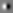
\includegraphics[width=0.15\columnwidth]{\figpath/Gx} &
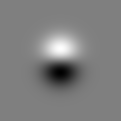
\includegraphics[width=0.15\columnwidth]{\figpath/Gy} &
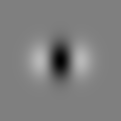
\includegraphics[width=0.15\columnwidth]{\figpath/Gxx} &
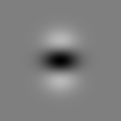
\includegraphics[width=0.15\columnwidth]{\figpath/Gyy} \\
(a) & (b) & (c) & (d) \\
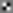
\includegraphics[width=0.15\columnwidth]{\figpath/Gxy} &

\includegraphics[width=0.15\columnwidth]{\figpath/Gxx-Gyy} &

\includegraphics[width=0.15\columnwidth]{\figpath/haar_sin} &

\includegraphics[width=0.15\columnwidth]{\figpath/haar_cos} \\
(e) & (f) & (g) & (h) \\
\end{tabular}
%
\caption{(a,b)~First derivatives, $\Gx$ and $\Gy$; (c-e)~Second derivatives, $\Gxx$, $\Gyy$ and $\Gxy$; (f)~$\Gxx-\Gyy$; (g,h)~Haar-like approximations to $\Gxy$ and $\Gxx-\Gyy$.}
\label{f:filters}
\end{figure}


\subsection{The Dual Tree Complex Wavelet Transform (\dtcwt{})}
Although filters based on second derivatives can give accurate output when positioned at the centre of a line feature, accuracy when away from the centre of the line cannot be assured. It has been noted, therefore, that accommodating variation in \emph{phase} of the filter can offer benefits in this regard. 

In particular, researchers have recognised the importance of using local phase information to distinguish between strong edges and genuine curvilinear structure. In mammography, examples include using Gabor filters~\cite{Rangayyan_Ayres_MBEC06}, while other studies used sets of complex filters~\cite{Schenk_Brady_IWDM02,McLoughlin_etal_SPIE02} that were also steerable~\cite{Freeman_Adelson_TPAMI91}, at multiple scales to compute local energy, orientation and phase at each pixel. One further study used the `monogenic' signal~\cite{Wai_etal_MICCAI04} as a more efficient way of calculating local phase and orientation at multiple scales, detecting curvilinear structure using amplitude-weighted local phase congruency. Overall, the conclusion that can be drawn from the literature is that the detection of curvilinear structure benefits from access to local phase and magnitude information at multiple scales.

An alternative to these methods is to use wavelets to describe the underlying image information. Wavelet transforms have been used extensively in image processing and analysis to provide a rich description of local structure. In particular, the Dual-Tree Complex Wavelet Transform (\dtcwt{}) gives a directionally selective representation that combines the computational efficiency of decimation (\ie~multiresolution filtering is achieved by successively down-sampling the image than by increasing filter size) with approximately shift-invariant coefficient magnitudes and local phase information~\cite{Kingsbury_ACHA01}. The \dtcwt{} combines the outputs of two discrete transforms, using real wavelets differing in phase by 90\deg, to form the real and imaginary parts of complex coefficients. For 2-D images, it produces six directional sub-bands, oriented at $\pm$15\deg, $\pm$45\deg and $\pm$75\deg, at each of a series of scales separated by factors of two. The DT-CWT is less expensive to compute and provides a richer description (magnitude and phase at six orientations rather than one) than the monogenic signal~\cite{Wai_etal_MICCAI04}.

Though it is easy to argue for the rich description of local structure provided by the \dtcwt{}, we must decide how to use this information to compute a single measure of curvilinear structure probability. One solution would be to select the maximum of the six oriented sub-band coefficients at each scale, and combine them across scale in a measure of phase congruency, as in the monogenic signal based method~\cite{Wai_etal_MICCAI04}, but this would discard potentially useful information. Instead, we pose the problem as a classification task in which we attempt to learn the patterns of DT-CWT coefficients associated with pixels belonging to either linear structures or background. 

We construct a feature vector characterising each pixel by sampling \dtcwt{} coefficients (in phase/magnitude form) from the six oriented sub-bands in each of the $s$ finest decomposition scales from a neighbourhood centred on the pixel. This involves interpolating the coefficients obtained at coarse scales to provide a response at every pixel using a band-pass interpolation method~\cite{Anderson_etal_ICIP05}. 

To improve further the rotational symmetry of the coefficients, we also apply an additional set of filters to reduce the wave frequencies of the 45\deg and 135\deg sub-bands so that they lie closer to the 15\deg, 75\deg, 105\deg and 165\deg bands~\cite{Kingsbury_ECSP06,Berks_etal_IPMI11}. The six sub-bands are then multiplied by \{$i$, -$i$, $i$, -1, 1, -1\} respectively, so that the phase at the centre of the impulse response of each wavelet is zero. Finally, to achieve 180\deg rotational symmetry, we replace any coefficient with negative imaginary part with its complex conjugate (equivalent to taking the absolute value of the local phase).

When dealing with a complex response, $c$, we separate its magnitude, $|c|$, from its phase, $\angle c$. Since orientation is only defined up to a rotation of $180^\circ$, however, a point with phase $\phi$ displaced by $d$ from the centre of a line is indistinguishable from a point with phase $-\phi$ displaced by $-d$ from the same line when looking in the opposite direction; we therefore take the absolute value of phase, $|\angle c|$, at each pixel.


\subsection{Multiresolution Filtering}
Since curvilinear structure appears at a number of scales in the image (\eg~from fine spicules to thick ducts in mammograms), it is also important to filter the image at several scales to capture all structure~\cite{Lindeberg_IJCV98b}. Having applied our filter bank at a number of scales, an important question is how to interpret the responses at each scale. One option is to discard all scales but that with the strongest overall response~\cite{Karssemeijer_teBrake_TMI96} and use the responses from the discrete orientations at the selected scale to determine orientation analytically. In this work, however, we investigate the alternative approach whereby we use the responses at all scales as input to a regressor that predicts the orientation directly. This general purpose approach has the added advantage that it can be applied for filter banks where an analytic solution is not obvious (such as the \dtcwt{}).